\section{Observed Trends}
\label{sec:observed-trends}

\textbf{RQ4:} \textit{What is the average skin-tone that is being observed progressively?}

In addition to visualizing the distribution of luminance across roles, we also explored broader temporal and structural patterns in skin tone representation using trend analysis and clustering techniques.

\subsection{Linear Trend of Luminance by Role Over Time}
\label{sec:linear-trend-luminance}
This plot shows the linear regression trend lines for average luminance values of different roles from 2019 to 2024. Each role was analyzed independently to assess whether skin tone preferences have shifted over time. The regression lines reveal relatively stable trends for most roles, with consistently higher luminance values for lead actors and actresses compared to their side-role counterparts.

\begin{figure}[!htpb]
    \centering
    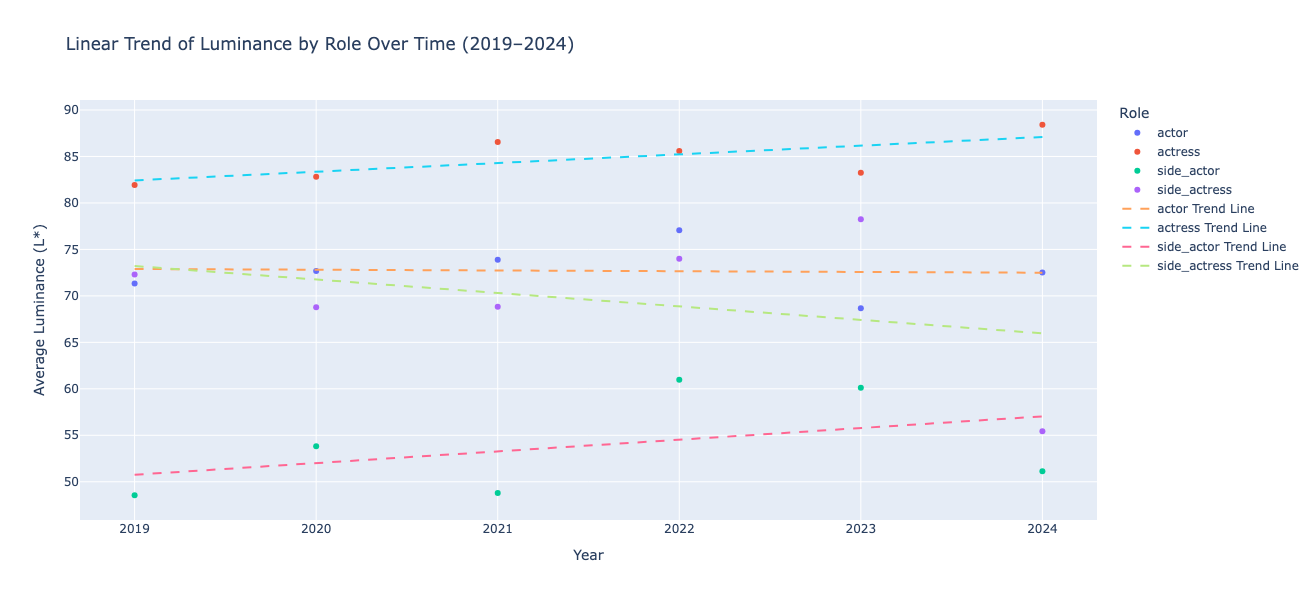
\includegraphics[width=0.8\textwidth]{linear_trand_of_luminance_by_role.png}
    \caption{\textit{Linear trend of luminance by role over time.}}
    \label{fig: Linear trend of luminance by role}
\end{figure}

\textit{This persistence of lighter skin tones in leading roles suggests an entrenched aesthetic preference that has remained largely unchanged in recent years}.

The regression coefficients for each role were calculated to quantify the rate of change in luminance over time. The results indicate that while \textit{the average luminance for lead roles remains high, the side roles exhibit a more pronounced increase in luminance, suggesting a potential shift toward more diverse casting choices in supporting characters.}

\begin{lstlisting}
Regression - Luminance over time:

                             OLS Regression Results                            
==============================================================================
Dep. Variable:                      L   R-squared:                       0.657
Model:                            OLS   Adj. R-squared:                  0.649
Method:                 Least Squares   F-statistic:                     93.17
Date:                Sun, 18 May 2025   Prob (F-statistic):           3.68e-44
Time:                        02:36:49   Log-Likelihood:                -708.79
No. Observations:                 200   AIC:                             1428.
Df Residuals:                     195   BIC:                             1444.
Df Model:                           4                                         
Covariance Type:            nonrobust                                         
==============================================================================
                coef    std err          t      P>|t|      [0.025      0.975]
------------------------------------------------------------------------------
Intercept    71.3063      1.199     59.461      0.000      68.941      73.671
C[actress]   11.9522      1.696      7.048      0.000       8.607      15.297
C[actor_s]  -20.0821      1.696    -11.841      0.000     -23.427     -16.737
C[actress_s] -2.2454      1.696     -1.324      0.187      -5.590       1.099
year_centered 0.5952      0.209      2.851      0.005       0.183       1.007
==============================================================================
Omnibus:                       97.570   Durbin-Watson:                   1.499
Prob(Omnibus):                  0.000   Jarque-Bera (JB):              882.950
Skew:                          -1.612   Prob(JB):                    1.86e-192
Kurtosis:                      12.775   Cond. No.                         12.6
==============================================================================
\end{lstlisting}

\subsection{K-Means Clustering of Skin Tone and Role}
To uncover hidden structures in the data, we applied K-means clustering to the luminance values, allowing the data to define natural groupings without preassigned labels. The clusters are visualized with respect to role categories and luminance levels.

\begin{figure}[!htpb]
    \centering
    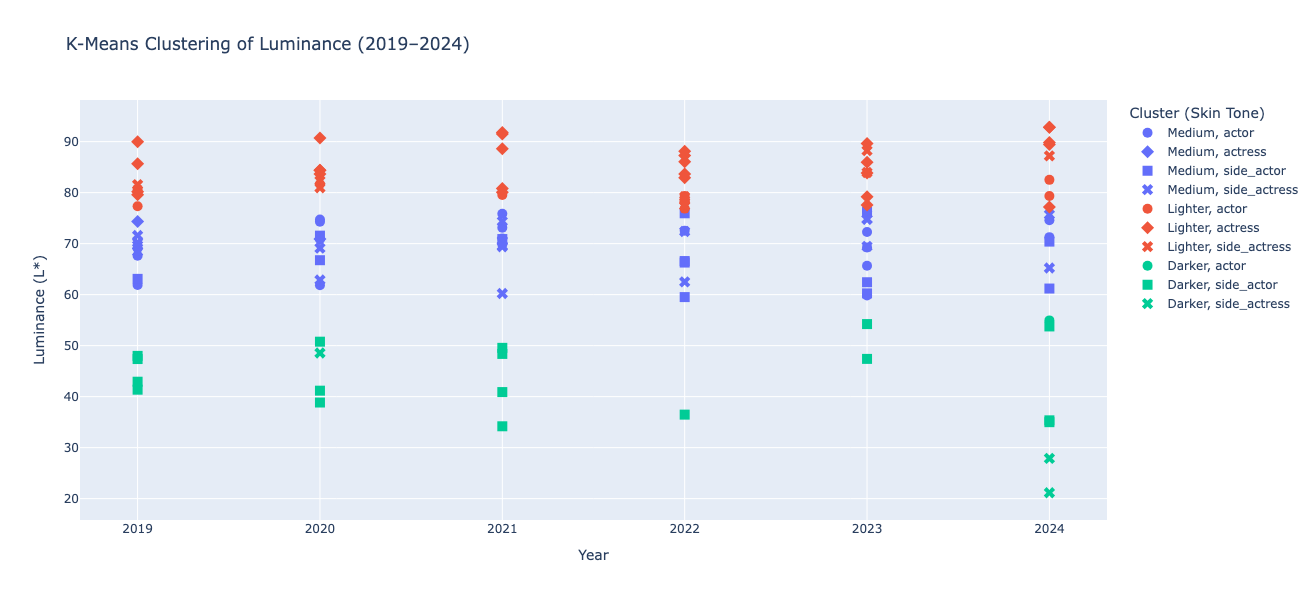
\includegraphics[width=0.8\textwidth]{k_means_clustering.png}
    \caption{\textit{K-means clustering of skin tone and role.}}
    \label{fig: K-means clustering of skin tone and role}
\end{figure}

\textit{The clustering reveals that roles often align with luminance-based groupings: lead roles predominantly fall into lighter-skin clusters, while side roles are more dispersed, including a larger proportion of darker-skin representations}. This unsupervised analysis reinforces the findings from earlier sections and highlights the stratification of skin tones by casting hierarchy.